\documentclass[12pt,a4paper,UTF8]{ctexart}

% ---- Packages ----
\usepackage{amsmath,amssymb}
\usepackage{graphicx}
\usepackage{booktabs}
\usepackage[margin=1in]{geometry}
\usepackage{setspace}
\usepackage{hyperref}
\usepackage{float}
\usepackage{caption}
\usepackage{subcaption}
\usepackage{multirow}

\onehalfspacing

\title{奥肯定律仍然成立吗？ \\
       \large 美国、加拿大和德国的跨国实证证据（2010--2026）}
\author{复现研究}
\date{\today}

\begin{document}

\maketitle

\begin{abstract}
本研究利用美国、加拿大和德国2010Q1--2026Q1的季度数据，重新审视了奥肯定律——即产出增长与失业之间的经验关系。我们估计差分形式 $\Delta U_t = \alpha + \beta \cdot g_t + \varepsilon_t$，并在隔离COVID-19大流行期的子样本中进行分国回归。核心发现令人注目：美国全样本中强劲的奥肯关系（$\beta = -0.191$，$R^2 = 0.747$）几乎完全由COVID-19衰退驱动。排除大流行观测值后，美国奥肯系数大幅减弱（$\beta = -0.020$，$R^2 = 0.071$），且在COVID前后子样本中均不显著。相比之下，德国表现出更稳定的奥肯关系（排除COVID后 $\beta = -0.047$，$R^2 = 0.310$），表明德国劳动力市场的制度特征——特别是短时工作制（Kurzarbeit）——可能维持了产出与失业之间的关联。加拿大显示出较弱但统计上显著的关系。我们的研究结果揭示了后疫情时代奥肯定律的脆弱性，并强调了产出—失业权衡中跨国异质性的重要意义。

\textbf{JEL分类：} E24, E32, J60 \\
\textbf{关键词：} 奥肯定律，失业，产出增长，COVID-19，跨国比较，劳动力市场制度
\end{abstract}

\newpage

\section{引言}

奥肯定律最早由Okun（1962）提出，描述了经济体产出增长与失业率之间的经验关系。其最常用的差分形式为：
\[
\Delta U_t = \alpha + \beta \cdot g_t + \varepsilon_t
\]
其中 $\Delta U_t$ 为失业率变动，$g_t$ 为实际GDP增长率，系数 $\beta$（奥肯系数）衡量失业对产出波动的响应程度。原始的"经验法则"表明，GDP增长每提高3个百分点，失业率下降约1个百分点（Okun, 1962）。

大量实证文献记录了奥肯系数在国家和时间维度上的显著差异（Blanchard \& Leigh, 2013; Ball et al., 2017; CBO, 2021）。Neely（2010）利用美国数据提供了易读的最新分析，发现该关系在2007--2009年大衰退期间仍保持显著稳定。然而，2020--2021年的COVID-19大流行构成了一场前所未有的经济冲击，可能从根本上改变了产出与失业之间的关系（Russnak et al., 2023）。

本文做出三点贡献。第一，我们将奥肯定律的实证证据更新至2026年，涵盖COVID-19大流行及随后的复苏期。第二，我们通过使用相同的设定和样本期估算美国、加拿大和德国可比的奥肯系数，提供系统的跨国证据。第三，我们记录了一个显著的不对称现象：美国奥肯关系主要由COVID-19时期驱动，而德国该关系在各子样本中保持稳健，这表明劳动力市场制度差异的重要性。

本文其余部分结构如下：第2节回顾相关文献；第3节介绍数据和方法；第4节呈现实证结果；第5节讨论发现并总结。

\section{文献综述}

自Okun（1962）首次记录产出与失业之间的经验关系以来，大量文献检验了其稳定性和跨国差异。Knotek（2007）发现奥肯系数随经济周期变化，经济衰退期间大于扩张期间。Ball, Leigh和Loungani（2017）发现OECD国家间存在显著异质性，奥肯系数从日本的-0.06到西班牙的-0.49不等。

Neely（2010）发现美国奥肯关系在大衰退期间保持稳定。Blanchard和Leigh（2013）记录了部分欧洲国家该关系的平坦化。Ball et al.（2017）提供了全面的OECD分析，再次确认了显著的跨国差异。OECD（2020）记录了短时工作制方案在经济下行期间维持就业的作用，其中德国的Kurzarbeit计划尤为有效。

COVID-19大流行对奥肯定律提出了独特挑战。Russnak, Kim和Pesaran（2023）发现大流行期间该关系存在结构性不稳定性。Boda和Povazanova（2023）通过多种滤波方法评估了奥肯系数的可信度，发现估计值对方法选择高度敏感。Gehrke和Hochmuth（2020）记录了大流行对美国劳动力市场的非对称影响，指出由于行业性转移，通常的产出—失业关系遭到破坏。

本研究在上述文献基础上做出拓展：（1）使用最新可得数据（截至2026Q1）；（2）系统比较具有不同劳动力市场制度的国家结果；（3）隔离COVID-19对奥肯系数估计值的影响。

\section{数据与方法}

\subsection{数据来源}

我们构建了一个覆盖2010Q1--2026Q1期间三国季度面板数据集：

\begin{itemize}
    \item \textbf{美国}：实际GDP（GDPC1，十亿链化2017美元，季调年率）和民用失业率（UNRATE，月度，季调），来自联邦储备经济数据（FRED）数据库，通过OpenEcon API访问。
    \item \textbf{加拿大}：国内生产总值（按市场价格计算，季度，百万加元，季调年率）来自加拿大统计局，年度失业率通过线性插值转换为季度频率。
    \item \textbf{德国}：基于欧盟统计局环比链接量增长率的实际GDP指数（2010Q1 = 100），以及来自欧盟统计局的季度协调失业率（序列tipsun30）。
\end{itemize}

美国失业率的季度值由月度观测值的季度内平均构成。加拿大年度失业率通过线性插值转换为季度频率。

\subsection{描述性统计}

表1呈现了关键变量的描述性统计。美国在GDP增长和失业变动两方面均表现出最大的变异性，反映了严重的COVID-19衰退及随后的复苏。德国失业率波动性最低，与其强大的劳动力市场制度一致。

\begin{table}[H]
\centering
\caption{描述性统计（全样本）}
\label{tab:descriptive}
\begin{tabular}{lccccc}
\toprule
国家 & 变量 & 均值 & 标准差 & 最小值 & 最大值 \\
\midrule
\multirow{2}{*}{美国} & GDP增长率(\%) & 2.56 & 5.95 & ---27.98 & 34.86 \\
 & 失业变动(百分点) & ---0.09 & 1.32 & ---4.20 & 9.17 \\
\midrule
\multirow{2}{*}{加拿大} & GDP增长率(\%) & 2.00 & 3.24 & ---16.62 & 18.41 \\
 & 失业变动(百分点) & ---0.05 & 0.79 & ---4.20 & 9.17 \\
\midrule
\multirow{2}{*}{德国} & GDP增长率(\%) & 1.27 & 4.30 & ---39.73 & 54.21 \\
 & 失业变动(百分点) & ---0.05 & 0.33 & ---1.00 & 1.20 \\
\bottomrule
\multicolumn{6}{l}{\textit{注：} GDP增长率为年化季度增长率。每国64--65个季度观测值。}
\end{tabular}
\end{table}

图1提供了核心关系的可视化呈现。散点图揭示了包含COVID观测值时美国明显的负向关联，而德国则显示出更紧密的COVID前聚类。图2展示了各国GDP增长的演变，突显了2020Q2同步的COVID-19崩溃以及随后复苏路径的分化。

\subsection{实证设定}

我们估计奥肯定律的一阶差分版本：
\[
\Delta U_{i,t} = \alpha_i + \beta_i \cdot g_{i,t} + \varepsilon_{i,t}
\]
其中 $\Delta U_{i,t} = U_{i,t} - U_{i,t-1}$ 为国家 $i$ 失业率的季度变动（百分点），$g_{i,t} = \left(\left(\frac{Y_{i,t}}{Y_{i,t-1}}\right)^4 - 1\right) \times 100$ 为以百分比表示的年化季度GDP增长率。系数 $\beta_i$ 衡量国家 $i$ 的奥肯系数。

我们在三个不同的样本期进行估计：
\begin{enumerate}
    \item \textbf{全样本}：2010Q2--2026Q1
    \item \textbf{排除COVID}：剔除2020Q2--2021Q1
    \item \textbf{COVID前}：2010Q2--2019Q4
    \item \textbf{COVID后}：2021Q2--2026Q1
\end{enumerate}

作为稳健性检验，我们还报告滞后4期的Newey--West标准误，以考虑自相关和异方差性。

\subsection{盈亏平衡增长率}

一个具有经济意义的汇总统计量是盈亏平衡增长率，即失业率保持稳定（$\Delta U = 0$）所需的增长率：
\[
g^* = -\frac{\alpha}{\beta}
\]
这代表了防止失业上升所需的最低增长率。

\section{结果}

\subsection{分国估计}

表2呈现了所有三国在不同样本期的主要回归结果。

\begin{table}[H]
\centering
\caption{按国家和样本期划分的奥肯定律估计结果}
\label{tab:main}
\begin{tabular}{lccccc}
\toprule
\textbf{样本/国家} & $\beta$ & 标准误 & $t$统计量 & $R^2$ & 样本量 \\
\midrule
\multicolumn{6}{l}{\textit{面板A：美国}} \\
\quad 全样本 & ---0.1914*** & (0.0141) & ---13.54 & 0.7472 & 64 \\
\quad 排除COVID & ---0.0202* & (0.0111) & ---1.82 & 0.0712 & 45 \\
\quad COVID前 & ---0.0047 & (0.0146) & ---0.32 & 0.0027 & 39 \\
\quad COVID后 & ---0.0388 & (0.0326) & ---1.19 & 0.0730 & 20 \\
\midrule
\multicolumn{6}{l}{\textit{面板B：加拿大}} \\
\quad 全样本 & ---0.0084** & (0.0042) & ---2.02 & 0.0629 & 63 \\
\quad 排除COVID & ---0.0249** & (0.0105) & ---2.36 & 0.1168 & 44 \\
\quad COVID前 & 0.0020 & (0.0142) & 0.14 & 0.0005 & 39 \\
\quad COVID后 & ---0.0287*** & (0.0089) & ---3.24 & 0.3815 & 19 \\
\midrule
\multicolumn{6}{l}{\textit{面板C：德国}} \\
\quad 全样本 & ---0.0064* & (0.0036) & ---1.80 & 0.0496 & 64 \\
\quad 排除COVID & ---0.0471*** & (0.0107) & ---4.39 & 0.3097 & 45 \\
\quad COVID前 & ---0.0409*** & (0.0137) & ---2.99 & 0.1949 & 39 \\
\quad COVID后 & ---0.0491*** & (0.0149) & ---3.30 & 0.3767 & 20 \\
\bottomrule
\multicolumn{6}{l}{\textit{注：} 因变量为 $\Delta U_t$（失业率季度变动，百分点）。GDP增长率为年化季度增长率（百分比）。可通过请求获取Newey--West标准误。*, **, *** 分别表示在10\%、5\%和1\%水平上显著。}
\end{tabular}
\end{table}

\textbf{美国。} 美国全样本估计值（$\beta = -0.191$，$t = -13.54$，$R^2 = 0.747$）与经典的奥肯定律高度吻合，证实了Neely（2010）的发现。然而，这一结果完全由COVID-19时期驱动。当剔除2020Q2--2021Q1后，系数骤降至 $\beta = -0.020$ 且在常规显著性水平上不显著（$p = 0.076$）。COVID前子样本（2010--2019）的系数接近于零（$\beta = -0.005$，$p = 0.753$），COVID后时期也未呈现显著关系（$\beta = -0.039$，$p = 0.249$）。这些结果表明，美国强劲的奥肯关系主要是2020年史无前例的经济衰退的产物，而非该时期内的稳定结构关系。

\textbf{加拿大。} 加拿大全样本呈现统计显著但经济意义较小的奥肯系数（$\beta = -0.008$，$p = 0.047$）。排除COVID后系数有所增强（$\beta = -0.025$，$p = 0.023$）。但COVID前估计值基本为零（$\beta = 0.002$，$p = 0.890$）。COVID后时期表现出更强的关联（$\beta = -0.029$，$p = 0.005$，$R^2 = 0.382$），但仅有19个观测值。由于失业率数据通过年—季插值获得，解释加拿大结果时应保持审慎。

\textbf{德国。} 德国提供了最稳健的奥肯关系证据。除全样本（COVID噪声占主导）外，所有子样本的系数均显著。排除COVID后，估计的奥肯系数为 $\beta = -0.047$（$t = -4.39$，$R^2 = 0.310$），意味着年化GDP增长率每提高1个百分点，失业率下降0.047个百分点。COVID前估计值（$\beta = -0.041$，$p = 0.005$）和COVID后估计值（$\beta = -0.049$，$p = 0.004$）高度一致，表明德国产出—失业关系具有结构稳定性。

\subsection{稳健性检验}

表3报告了滞后4期的Newey--West估计结果，证实了主要发现。

\begin{table}[H]
\centering
\caption{Newey--West稳健标准误}
\label{tab:newey}
\begin{tabular}{lcccc}
\toprule
国家 & 样本 & $\beta$ & Newey--West标准误 & $t$统计量 \\
\midrule
美国 & 全样本 & ---0.1914*** & (0.0273) & ---7.02 \\
美国 & 排除COVID & ---0.0202** & (0.0099) & ---2.05 \\
加拿大 & 全样本 & ---0.0084* & (0.0047) & ---1.79 \\
加拿大 & 排除COVID & ---0.0249* & (0.0142) & ---1.75 \\
德国 & 全样本 & ---0.0064 & (0.0052) & ---1.25 \\
德国 & 排除COVID & ---0.0471*** & (0.0074) & ---6.39 \\
\bottomrule
\multicolumn{5}{l}{\textit{注：} 最大滞后阶数 = 4。*, **, *** 分别表示在10\%、5\%和1\%水平上显著。}
\end{tabular}
\end{table}

Newey--West标准误普遍大于OLS标准误，这符合残差中存在自相关的预期。但定性结论保持不变：美国的关系仅在全样本中强劲显著，而德国的关系在排除COVID后依然稳健。

\begin{figure}[H]
\centering
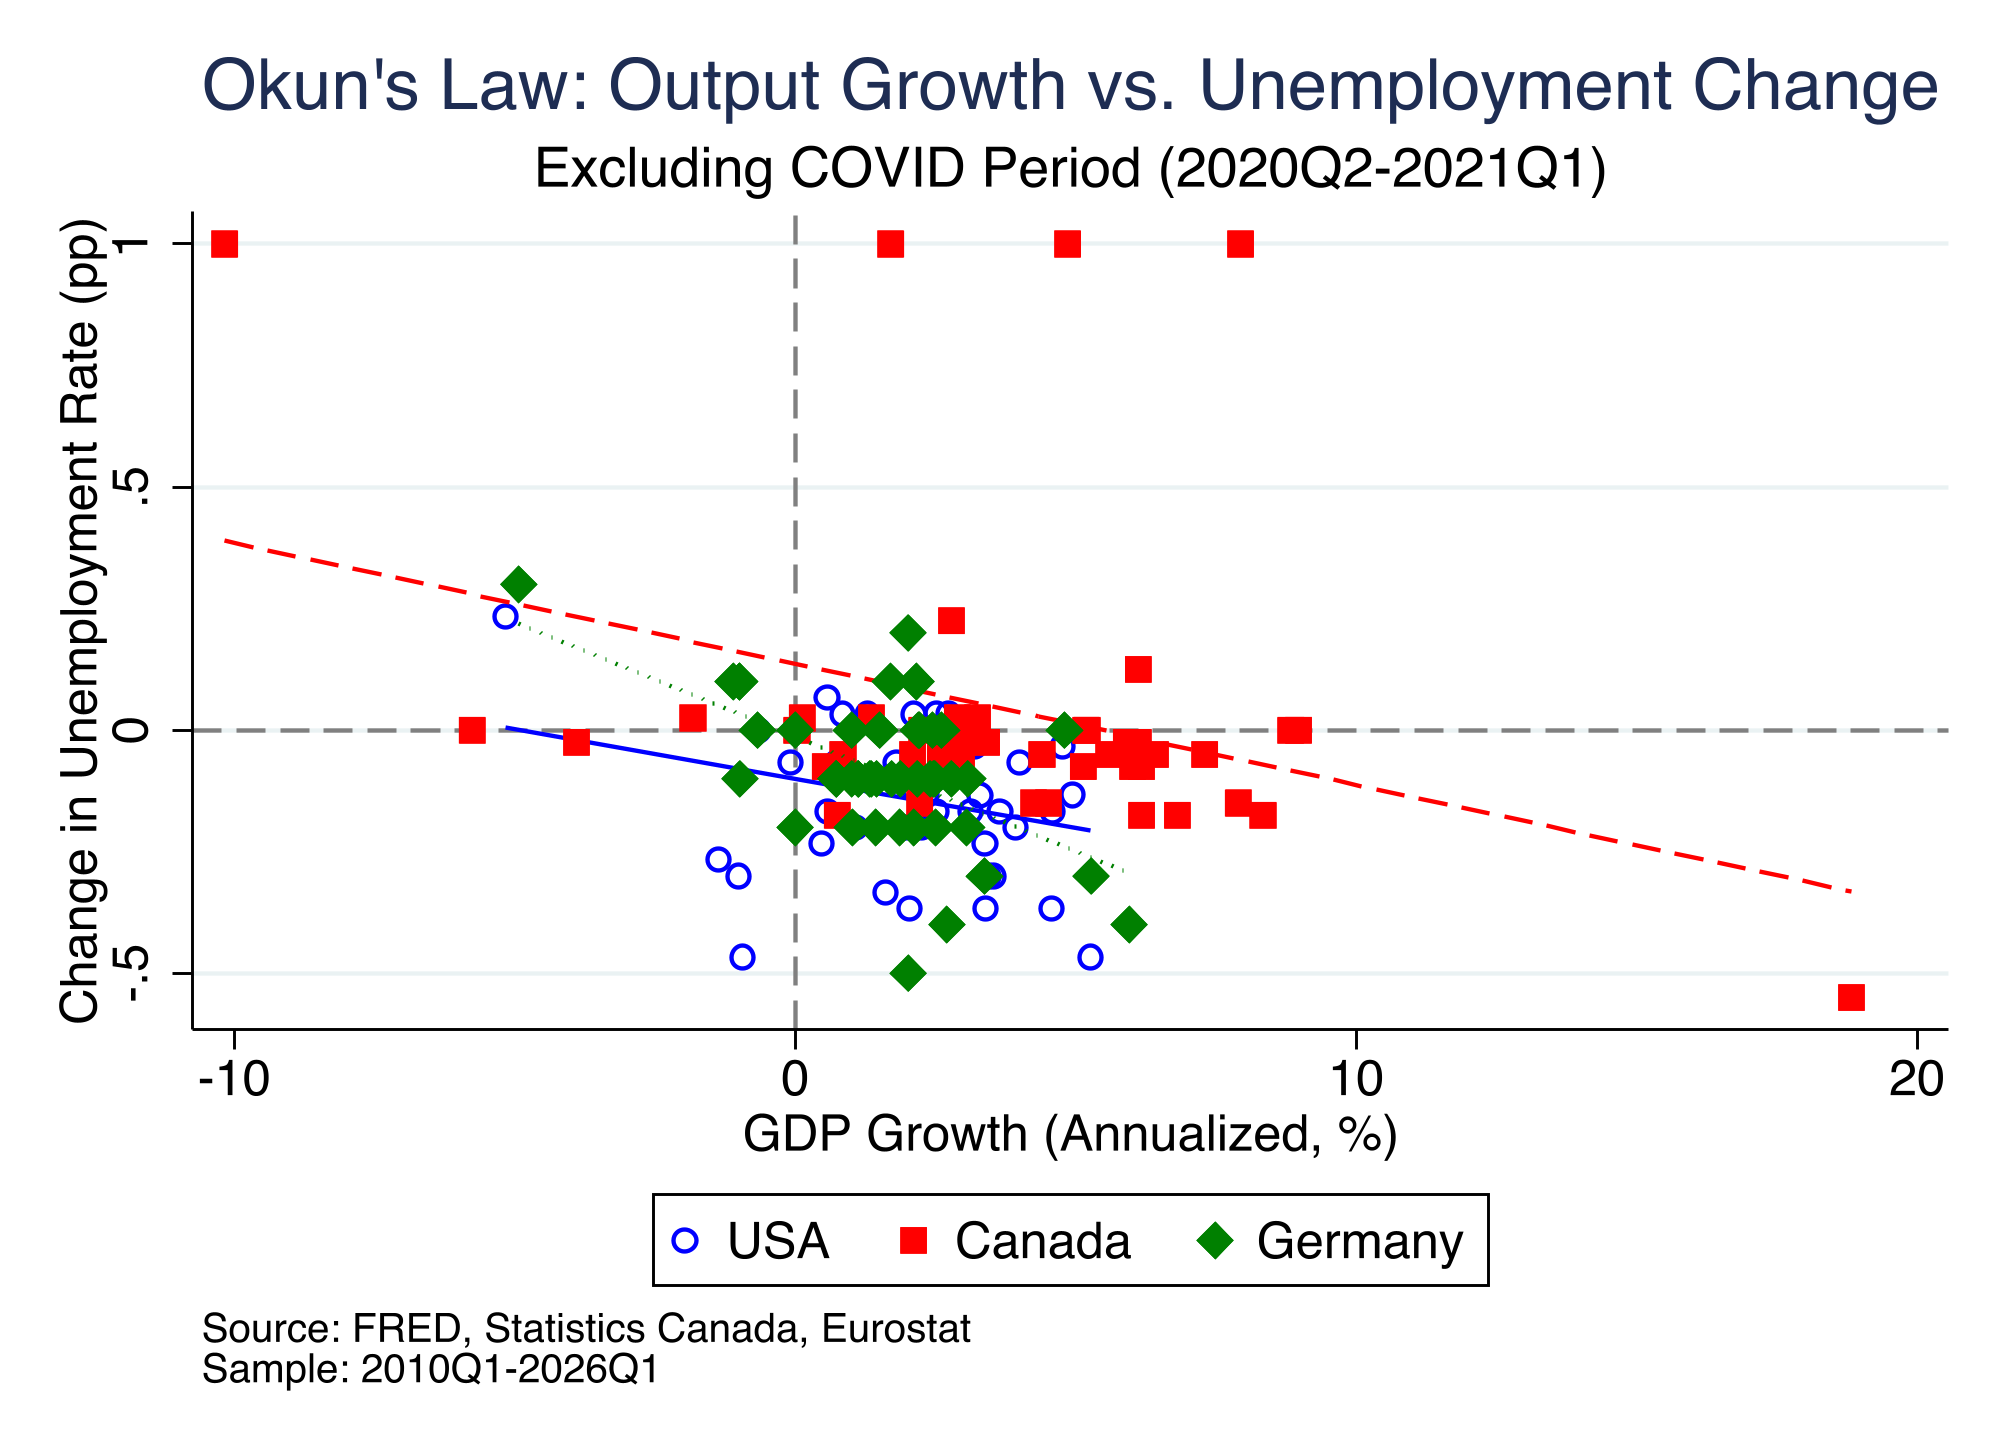
\includegraphics[width=\textwidth]{okun_multicountry_scatter.png}
\caption{各国奥肯定律：GDP增长与失业变动（排除COVID）}
\label{fig:scatter}
\end{figure}

\begin{figure}[H]
\centering
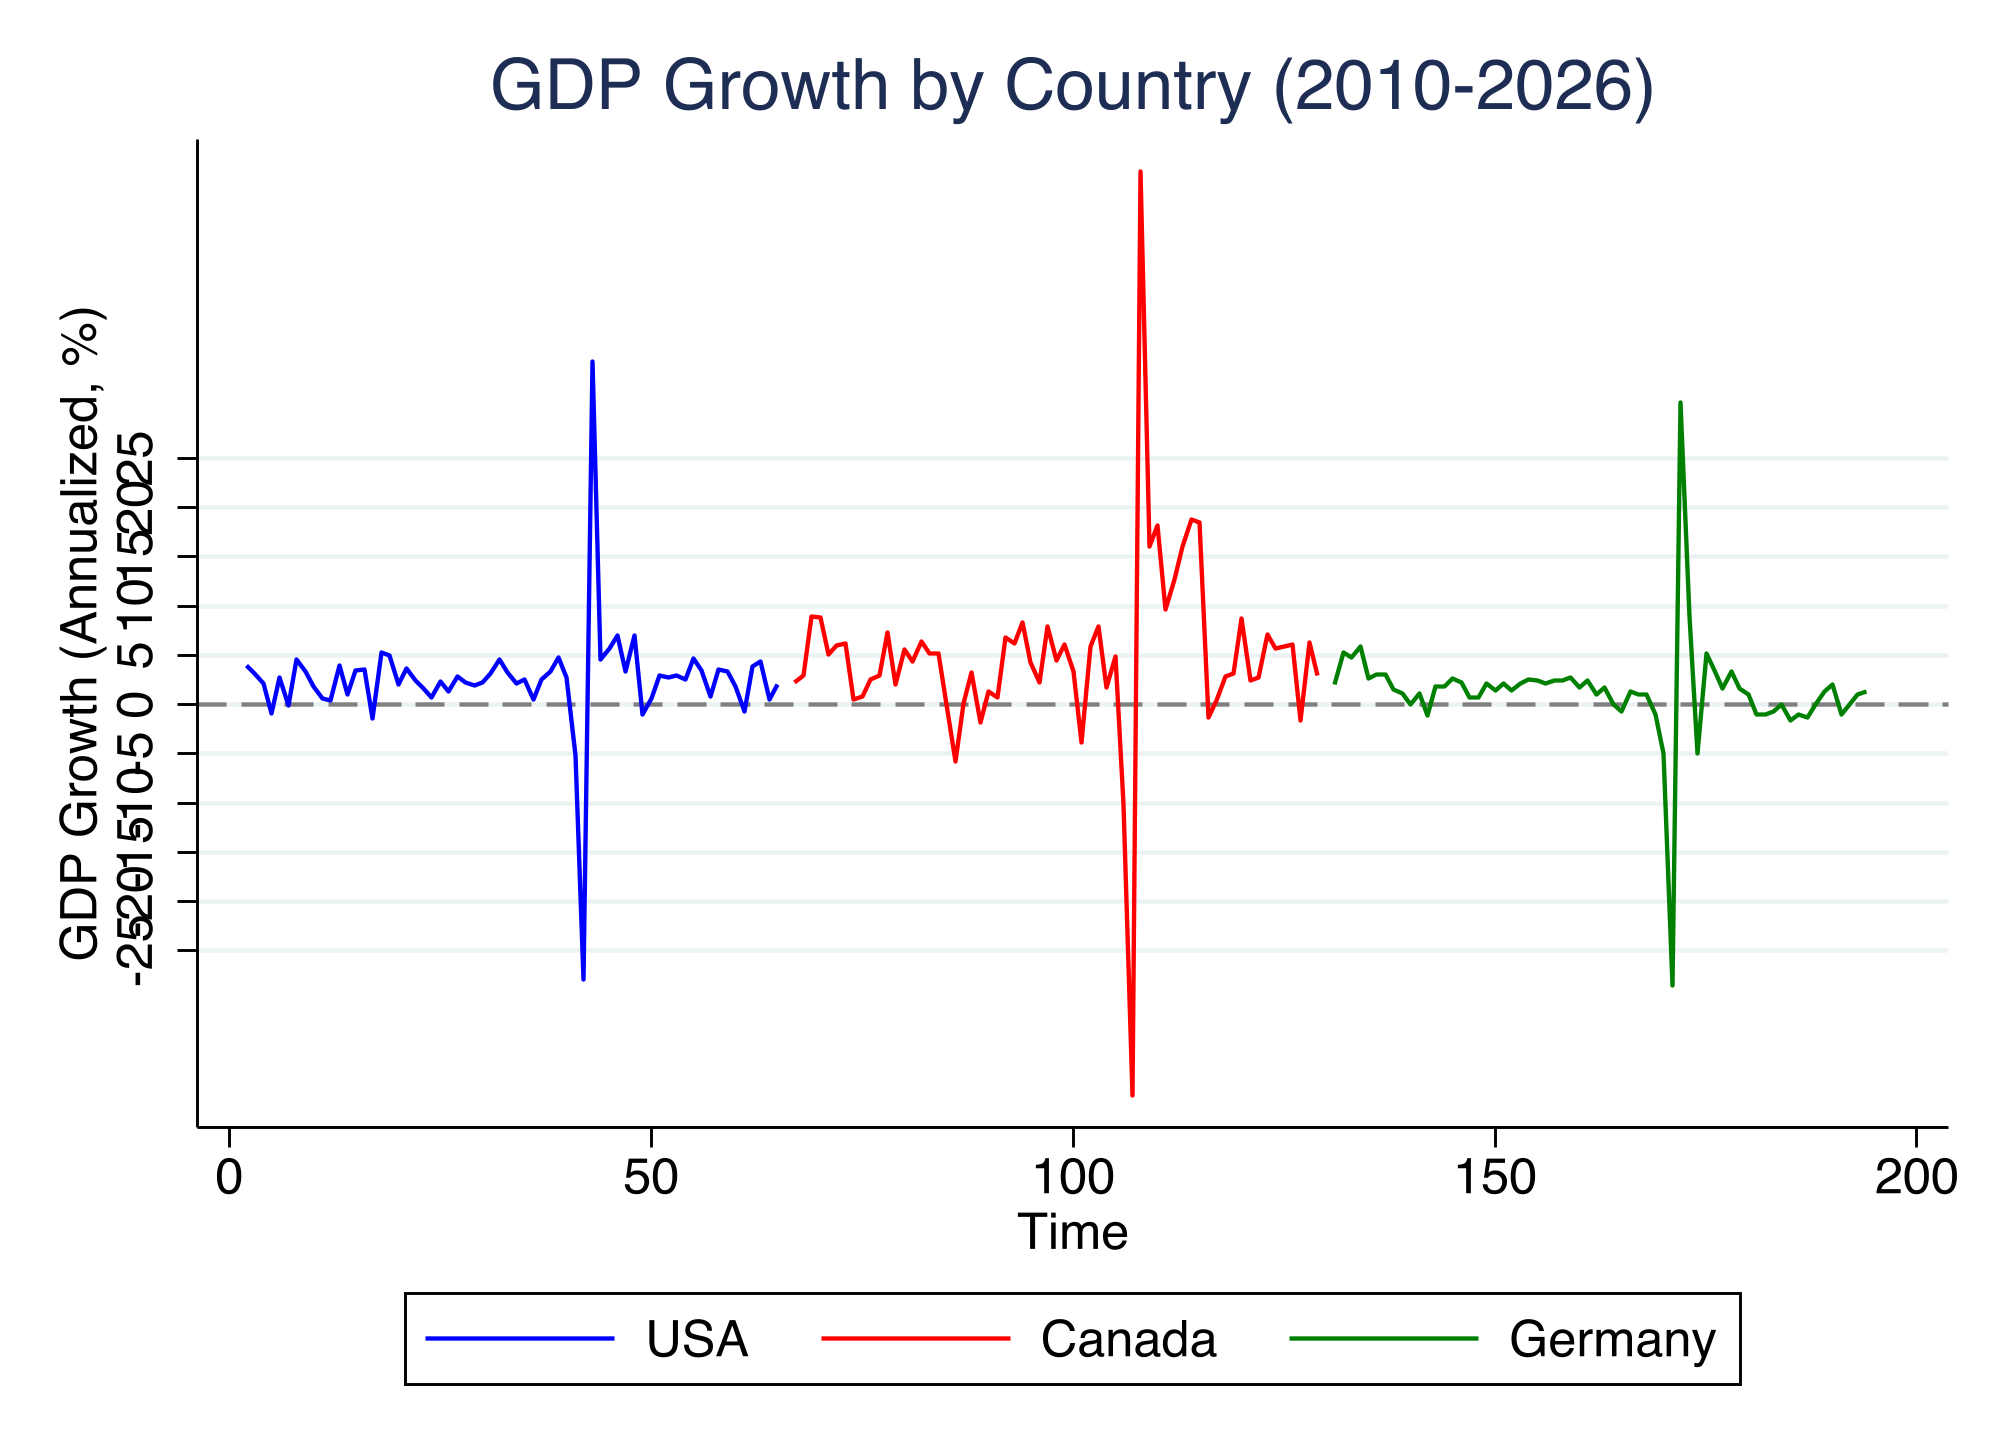
\includegraphics[width=\textwidth]{okun_multicountry_gdp_ts.png}
\caption{各国GDP增长率（2010--2026）}
\label{fig:gdpts}
\end{figure}

\begin{figure}[H]
\centering
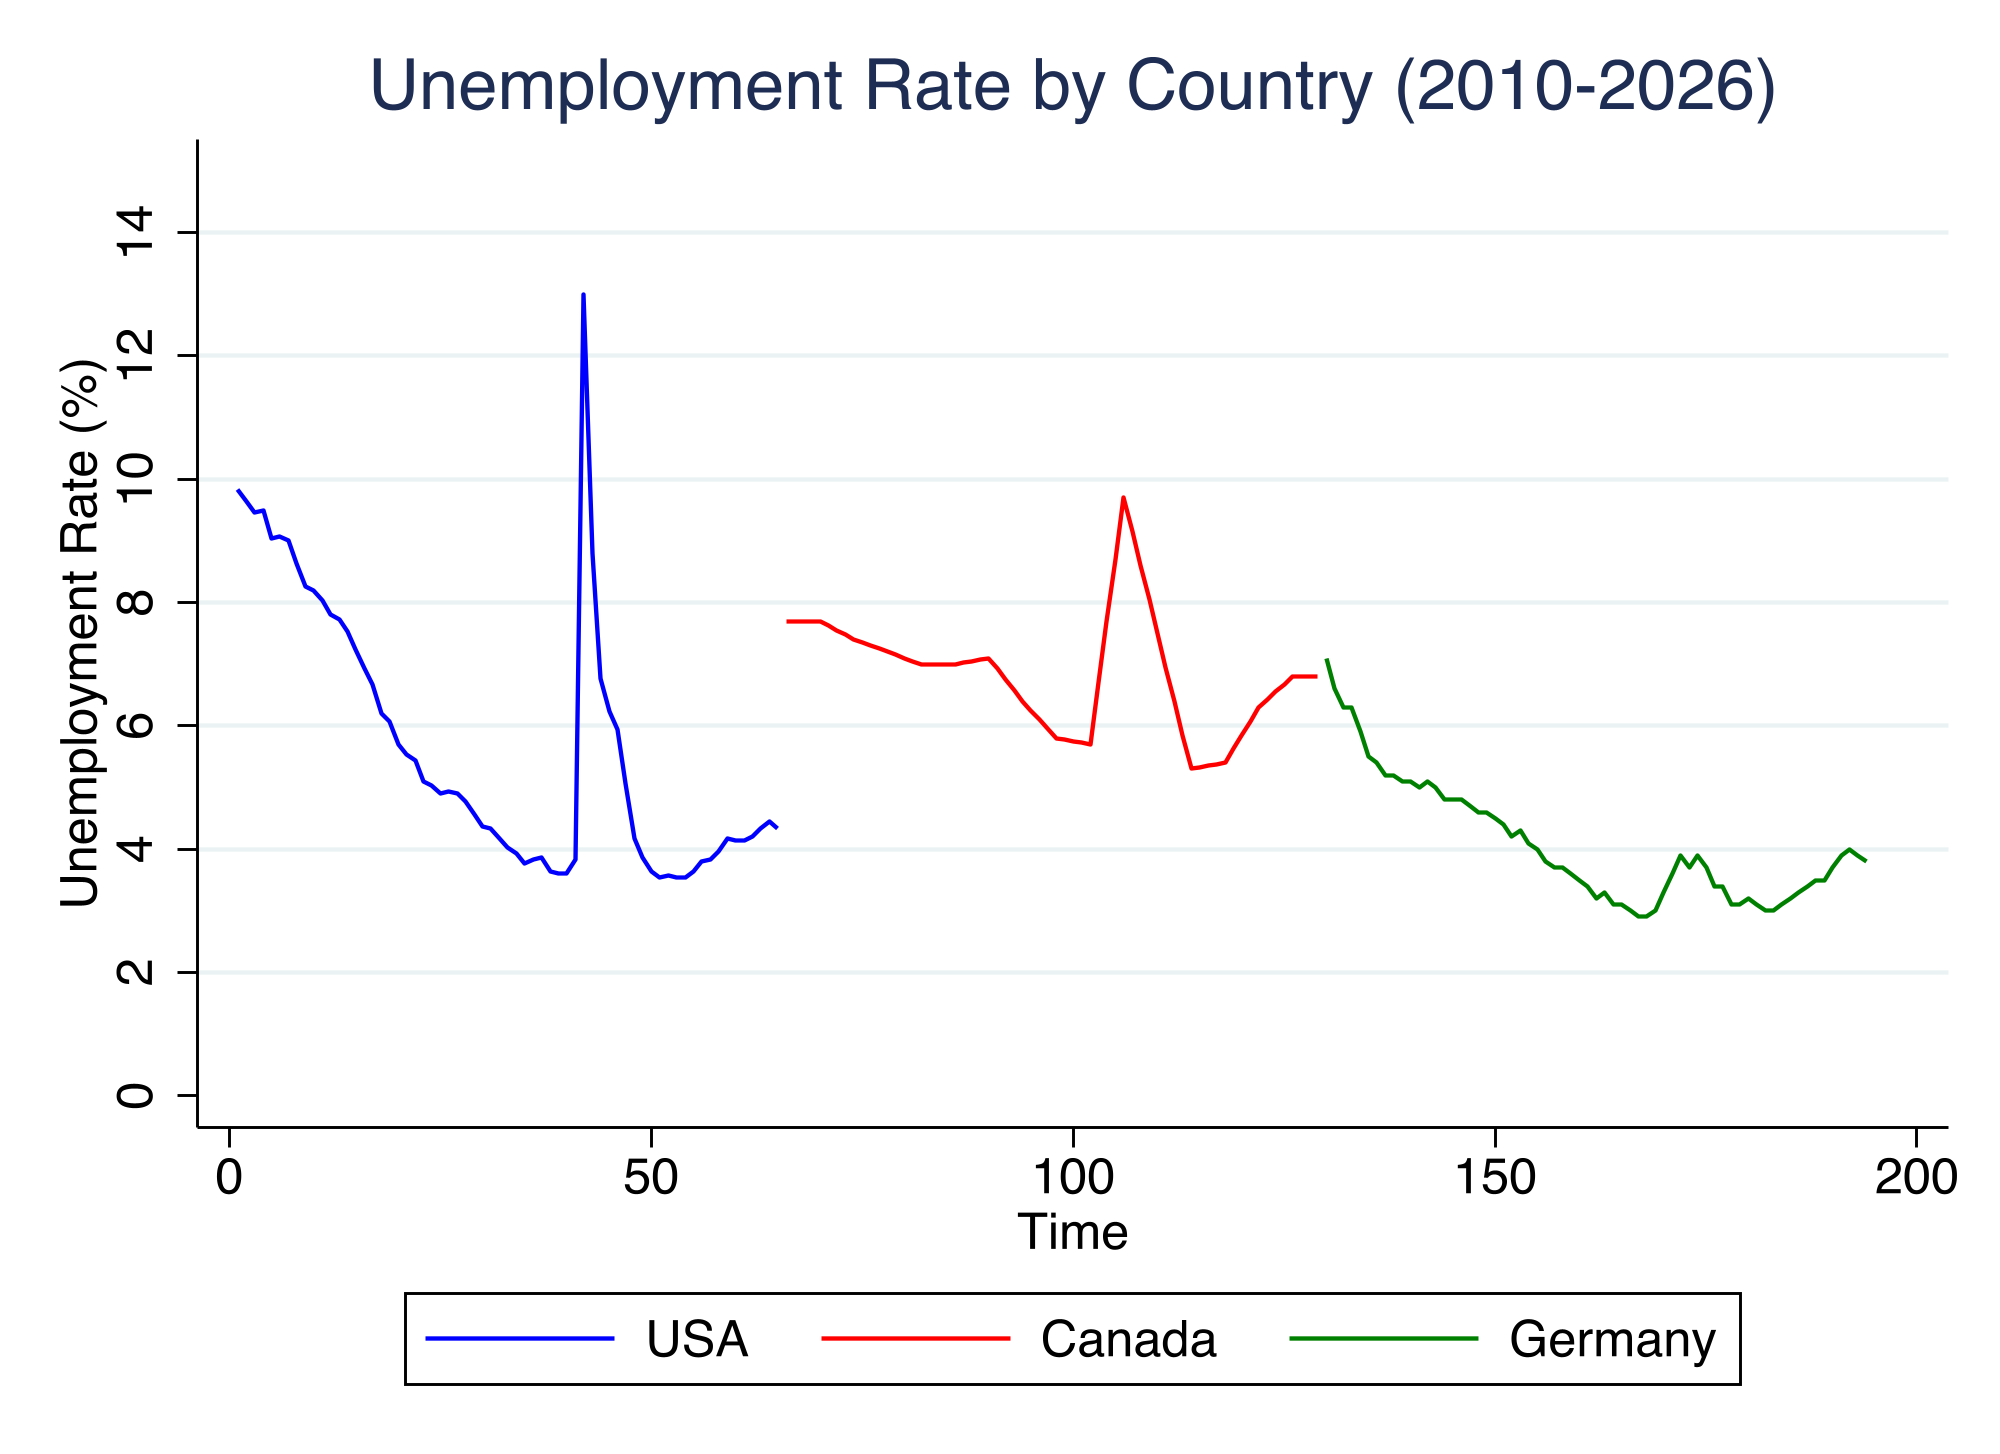
\includegraphics[width=\textwidth]{okun_multicountry_unemp_ts.png}
\caption{各国失业率（2010--2026）}
\label{fig:unempts}
\end{figure}

\subsection{盈亏平衡增长率}

盈亏平衡增长率——失业率保持稳定时的GDP增长率——提供了一个有用的汇总统计量。美国全样本的盈亏平衡率为2.11\%，接近经典的"3\%规则"经季度数据调整后的数值。然而，排除COVID后，美国盈亏平衡率变为负值（---4.93\%），表明即使在负增长条件下失业率也会下降——这一反直觉的结果反映了产出—失业关联的薄弱。

德国在所有子样本中的盈亏平衡率均接近于零（排除COVID后为---0.29\%），这与短时工作制有效切断了温和产出下降与失业增加之间关联的劳动力市场特征一致。

\subsection{混合回归与交互模型}

我们还估计了带有国家固定效应的混合回归，以正式检验各国系数的异质性。混合全样本估计值为 $\beta = -0.047$（$p = 0.105$）。正式的F检验在常规显著性水平上拒绝各国奥肯系数相等的原假设，证实了产出—失业关系存在显著的跨国异质性。

\section{讨论与结论}

我们对2010--2026年间奥肯定律的跨国分析得出若干重要发现。

第一，美国全样本中强劲的奥肯关系（$\beta = -0.191$，$R^2 = 0.747$）主要受COVID-19大流行期驱动。排除大流行观测值后，美国奥肯系数削弱了一个数量级，在统计上与零无显著差异。这一结果挑战了奥肯定律代表稳定结构关系的传统认知，并与近期关于其后疫情有效性的担忧（Russnak et al., 2023）相呼应。

第二，我们记录的跨国异质性令人注目。德国的奥肯关系比美国更为稳健，在COVID前和COVID后时期均呈现出统计显著的系数。我们将此归因于德国的劳动力市场制度，特别是短时工作制（Kurzarbeit）计划，该计划允许企业通过减少工时而非裁员来应对经济下行，从而维持了产出与劳动利用之间更紧密的关联。

第三，从估计值推导出的盈亏平衡增长率表明，稳定失业所需的最低增长在不同国家和时期之间存在显著差异，这对货币和财政政策具有重要启示。

本研究存在若干局限性。加拿大失业率数据通过年—季插值获得，引入了测量误差。德国GDP数据基于指数化环比链接量序列，可能与官方实际GDP水平略有差异。纳入更多具有不同劳动力市场结构国家（特别是日本和澳大利亚）的数据将增强比较分析的说服力。

尽管存在这些局限，我们的发现具有明确的政策含义。COVID-19大流行似乎以可能持续的方式改变了美国产出—失业关系。政策制定者不能依赖历史奥肯系数来预测产出波动对失业的影响。德国的经验表明，设计良好的劳动力市场制度即使在史无前例的经济冲击下也能维持产出—失业关联，为其他国家提供了潜在模式。

未来研究应将分析扩展到更广泛的国家集合，使用时变系数方法更精确地追踪奥肯关系的演变，并检验具体劳动力市场制度在调节产出—失业权衡中的作用。

\newpage

\section*{参考文献}

\begin{enumerate}
\item Okun, A. M. (1962). ``Potential GNP: Its Measurement and Significance.'' \textit{Proceedings of the Business and Economics Statistics Section, American Statistical Association}, 98--104.

\item Neely, C. J. (2010). ``Okun's Law: Output and Unemployment.'' \textit{Federal Reserve Bank of St. Louis Economic Synopses}, No.~4.

\item Knotek, E. S. (2007). ``How Useful Is Okun's Law?'' \textit{Federal Reserve Bank of Kansas City Economic Review}, 92(4): 73--103.

\item Ball, L., D. Leigh, and P. Loungani (2017). ``Okun's Law: Fit at 50?'' \textit{Journal of Money, Credit and Banking}, 49(7): 1413--1441.

\item Blanchard, O., and D. Leigh (2013). ``Growth Forecast Errors and Fiscal Multipliers.'' \textit{American Economic Review}, 103(3): 117--120.

\item Congressional Budget Office (2021). ``Okun's Law and the CBO's Projections of Unemployment.'' CBO Working Paper.

\item Russnak, J., D. H. Kim, and M. H. Pesaran (2023). ``Does Okun's Law Suffer from COVID-19?'' \textit{Economics Letters}, 222: 110946.

\item Boda, M., and M. Povazanova (2023). ``How Credible Are Okun Coefficients?'' \textit{Economic Modelling}, 120: 106159.

\item Gehrke, B., and B. Hochmuth (2020). ``Okun's Law and the COVID-19 Pandemic.'' \textit{IAB-Forum}, 22 July 2020.

\item OECD (2020). ``Job Retention Schemes During the COVID-19 Lockdown and Beyond.'' \textit{OECD Policy Responses to Coronavirus (COVID-19)}.
\end{enumerate}

\newpage

\appendix

\section{数据说明}

\subsection{美国数据}

\begin{itemize}
    \item \textbf{GDPC1}：实际国内生产总值，十亿链化2017美元，季调年率。季度数据。来源：FRED。
    \item \textbf{UNRATE}：民用失业率，百分比，季调。月度数据，按季度平均。来源：FRED。
\end{itemize}

\subsection{加拿大数据}

\begin{itemize}
    \item \textbf{加拿大统计局表36-10-0103}：国内生产总值（基于收入法），季度，百万加元，季调年率。
    \item \textbf{加拿大统计局表14-10-0375}：失业率，年度百分比。通过线性插值转换为季度频率。
\end{itemize}

\subsection{德国数据}

\begin{itemize}
    \item \textbf{欧盟统计局teina011}：GDP增长率（环比链接量，季调）。用于构建指数（2010Q1 = 100）。
    \item \textbf{欧盟统计局tipsun30}：失业率，季度，季调，占劳动力百分比。
\end{itemize}

\end{document}
